\documentclass[UTF8]{gapd}
\usepackage{amsmath} \usepackage{amssymb} \usepackage{booktabs}
\usepackage{diagbox}
\usepackage{float}
%基础模板,引用自GitHub: https://github.com/RocketshipGames/gapd.cls

% ■ ■ ■ ■ ■ ■ ■ ■ ■ ■ ■ ■ ■ ■ ■ ■ ■ ■ ■ ■ ■ ■ ■ 
% ■ ■ ■ ■ ■ ■ ■ ■ ■ ■ ■ ■ ■ ■ ■ ■ ■ ■ ■ ■ ■ ■ ■
% ■ ■               注意事项                 ■ ■
% ■ ■      不要瞎几把模板里面cls文件!!!!!   ■ ■
% ■ ■      写着不需要改动的地方别瞎几把动!!!   ■ ■
% ■ ■      有不懂的地方就直接联系编辑!!!!!   ■ ■
% ■ ■      不要自作主张!!!!!!             ■ ■
% ■ ■      否则后续排版会非常累的!!!!!!!   ■ ■
% ■ ■ ■ ■ ■ ■ ■ ■ ■ ■ ■ ■ ■ ■ ■ ■ ■ ■ ■ ■ ■ ■ ■
% ■ ■ ■ ■ ■ ■ ■ ■ ■ ■ ■ ■ ■ ■ ■ ■ ■ ■ ■ ■ ■ ■ ■

%标题部分=================================================================
%上标(不需要改动!!!!)
\Type{Article}

%标题
\Title{
  圆柱形骰子
}

\CAuthor{谭帆驰,鲍子龙,丁俊翔}{IBPE2021}%显示于题目下的作者名,
\Author{Xing Ming}{}
%出现于页脚初的英文名,按“姓 名”的顺序写拼音

%摘要
\Abstract{本文是对2022CUPT第七题研究成果的一个总结.理论上,考虑了五种可能的计算概率的模型,重点分析了简单弹跳模型,将骰子的可能的运动学过程映射到了相空间中,通过临界条件确定的面积与相空间总面积的比值计算概率.最后将五种模型进行对比,利用最大似然估计,计算五种模型的似然函数,来判断哪一种模型更为可靠.实验上,采用随机投掷的方法进行投掷,对五种不同的材料进行了投掷.}
\Keywords{简单弹跳模型,相空间,最大似然估计,随机投掷.}
%编号与页码(以下两行不需要改动)
\Issue{1}{1}{2022}
\Pages{1}{3}%37
%不要改这里,好吗?

%正文部分=================================================================
\begin{document}
%\begin{CJK}{UTF8}{gbsn}
\maketitle

%一些常用的Latex语句:
%插入斜体:\textit{}
%引用文字:\begin{quote} \end{quote}
%插入脚标: \footnote{}

\section{简介}
\label{sec:Introduction}
To land a coin on its side is often associated with the idea of a rare occurrence. What should be \textbf{the physical and geometrical characteristics} of a cylindrical dice so that it has the \textbf{same probability} to land on its \textbf{side and one of its faces}?

一枚硬币落地时侧面站立的情况通常是很罕见的.为了使一个\textbf{圆柱形骰子}落下时能有\textbf{相同的概率}立在它的\textbf{侧面和上下表面其中之一},它应该具有怎样的\textbf{物理和几何特征}?

%插入普通图片
\iffalse
\begin{figure}[!htbp]%
  \centering
  \includegraphics[width=0.8\columnwidth]{图片地址}
  \caption{图片名}
  \label{fig:P2}%\label置于\caption后,否则可能报错
\end{figure}
\fi%实际写时不需要\iffalse \fi,(该组命令是为了编辑时不报错)

%插入跨列图片
\iffalse
\begin{figure*}[!htbp]
  \centering
  \includegraphics[width=1\linewidth]{图片地址}
  \caption{图片名}
  \label{fig:P1}
\end{figure*}
\fi

%插入图表一定要注意规范!!!!!!!!!!!!!!!!!!!!!!!!!!!!!!!!!!!!!!
%表格一律用三线表,如果有出现数据,请注明数据的单位,另外表格的标题等也要注明清楚。

%插入任何非原创图片都应当注意注明出处
%插入一般的曲线图,一定要注明坐标轴的含义!!!!!及其单位!!!!!!  格式一律为:      物理量 (单位)
%                                                                              ^
%                                                                              |
%                                                                              |
%                                                                              |
%                                                                例子:         ——————————————————————————>
%                                                                                     摆线长度  (mm)
%当图中存在多个曲线,或者数据与拟合图同时存在时,要写清楚图例!!!!!!!!!
%要善于运用跨列图片,把多个相似的子图拼组合成一张比较大的跨列图片


\section{理论}
\label{sec:Theory}
在介绍理论之前,先提出我们对理论做出的6条简化假设:
\begin{enumerate}
	\item 相空间的概率分布是均匀的
	\item 骰子质量分布均匀
	\item 忽略地面摩擦力与空气阻力
	\item 不考虑骰子两头同时着地的情况
	\item 与地面碰撞的时间可忽略不计
	\item 侧面与底面与地面碰撞的恢复系数一致
\end{enumerate}
在列举我们要说的模型之前,我们需要先设定一些参数,方便我们接下来的分析:
\begin{figure}[h]%
	\centering
	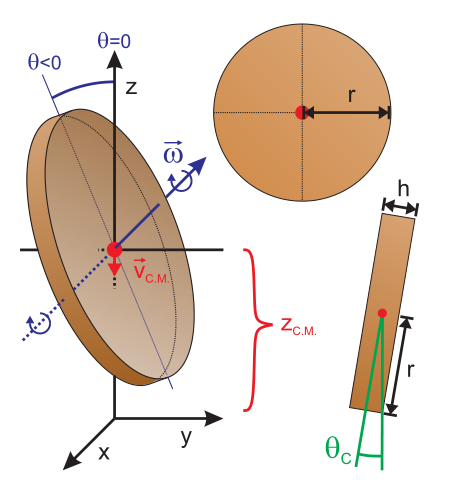
\includegraphics[width=0.8\columnwidth]{images/骰子2}
	\caption{参数图\cite{c3}}
	\label{fig:P2}%\label置于\caption后,否则可能报错
\end{figure}


高度与半径之比:\quad$\eta =\frac{h}{r}$

圆柱的对角线长度:\quad$l=\sqrt{r^2+(h/2)^2}$

角度c:\quad$\theta_{c}  = \arctan (\eta /2)$

线速度与角速度:\quad $v\quad and \quad\omega $

骰子的长轴与$z$轴所成角度:\quad$\theta$

质心与地面的高度:\quad$Z_{C.M.}$

\subsection{模型1-4}
模型一:表面面积之比求解概率(假设概率与面积成正比).
\begin{equation}
{p_{edge}}(h,r) = \frac{{2\pi rh}}{{2\pi {r^2} + 2\pi rh}} = \frac{\eta }{{1 + \eta }}
\end{equation}
模型二:横截面长度之比(假设概率与横截面长度成正比).
\begin{equation}
{p_{edge}}(h,r) = \frac{h}{{2(2r) + h}} = \frac{\eta }{{4 + \eta }}
\end{equation}
模型三:立体角之比求概率.假设在三面硬币的给定面上着陆的概率与该面所含的立体角成正比.
\begin{equation}
p_{edge}=\frac{\int_0^{2\pi}{\int_{\pi /2-\theta _c}^{\pi /2+\theta _c}{\sin \theta d\theta d\phi}}}{4\pi}=\sin \theta _c=\frac{\eta}{\sqrt{\eta ^2+4}}
\end{equation}
模型四:质心.

硬币与$z$轴所成的角度$\theta$将完全决定最终的静止形态:

1.如果      $0<\theta<\theta_{c}$           ,则硬币将落在侧面.

2.如果$\theta_{c}<\theta<\frac{\pi}{2}$,那么硬币将落在正面/反面.
\begin{equation}
{p_{edge}} = \frac{2\theta _c}{\pi}
\end{equation}

\subsection{模型5:简单弹跳模型}
简单反弹模型考虑了反弹的影响.反弹以以下方式进行.每次骰子与地面发生碰撞,与地面所接触的法向速度满足以下条件:
\begin{equation}
u''=-\gamma u'
\end{equation}


骰子的势能完全由高度 $z$ 决定,即  $U=mgz$             ,动能考虑其平动能以及转动能,得到:
\begin{equation}
T=\frac{m v^{2}}{2}+\frac{I_{x x} \omega^{2}}{2}
\end{equation}
其中:$I_{xx}=\frac{1}{4}mr^2+\frac{1}{12}mh^2$.

定义碰撞前瞬间的势能为最小势能,即:$U_{\min}\left( \theta \right) =mgz_{\min}\left( \theta \right) $             ,由几何关系可求得:
\begin{equation}
\begin{aligned}
z_{\min }(\theta) &=\sqrt{r^{2}+(h / 2)^{2}} \cos \left(|\theta|-\arctan \left(\frac{h}{2 r}\right)\right) \\
&=z^{*} \cos \left(|\theta|-\theta_{c}\right)
\end{aligned}
\end{equation}
定义骰子无法再次弹起的临界能量$E_{c}$:
\begin{equation}
E_{c}=mgz^*
\end{equation}
由于在最后一次碰撞中, $\theta$   的值不会发生瞬时变化,即在碰撞前的瞬间的状态已经决定了骰子的最终状态(i.e $-\theta _c\leqslant \theta \leqslant \theta _c$会落在边缘)

其中  $z^*$  是半对角线长度.

由(5)可得:
\begin{equation}
\Delta u=-(1+\gamma) u^{\prime}
\end{equation}
其中   $u'$  和 $u''$    代表碰撞前后竖直方向的速度.

另一方面,垂直方向的速度还可能与质心速度以及角动量的变化相关:
\begin{equation}
\Delta u=\Delta v+y(\theta) \Delta \omega
\end{equation}
其中   $y(\theta)$    代表质心与碰撞点连线的距离在水平方向的投影.

我们对碰撞点选择一个平行于 $x$  轴的参考轴,对该参考轴应用角动量守恒,得到:
\begin{equation}
m\left( -y \right) \varDelta v+I\varDelta \omega =0
\end{equation}
结合上述的(9),(10),(11),我们得到了质心速度与角速度的变化值:
\begin{equation}
\Delta v=-(1+\gamma) \cdot \frac{I}{I+m y^{2}}\left(v^{\prime}+y \omega^{\prime}\right)
\end{equation}
\begin{equation}
\Delta \omega=-(1+\gamma) \cdot \frac{m y}{I+m y^{2}}\left(v^{\prime}+y \omega^{\prime}\right)
\end{equation}
结合上述(12),(13),可得到能量的变化量:
\begin{equation}
\Delta E=-\frac{1-\gamma^{2}}{2} \cdot \frac{m I}{I+m y^{2}}\left(v^{\prime}+y \omega^{\prime}\right)^{2}
\end{equation}
接下来我们考虑临界碰撞状态需要满足的3个条件:
\begin{enumerate}
	\item 碰撞前的能量必须大于或等于  $E_{c}$   .
	\item 碰撞后的能量必须低于 $E_{c}$    .
	\item 由于物理约束,   $u'$ 必须为负值(方向向下).
\end{enumerate}
可写成3个数学表达式:
\begin{equation}
E^{\prime}(\theta, v, \omega) \geq E_{c}
\end{equation}
\begin{equation}
E_{c}>E^{\prime \prime}(\theta, v, \omega)=E^{\prime}(\theta, v, \omega)+\Delta E
\end{equation}
\begin{equation}
v^{\prime}+y \cdot \omega^{\prime}<0
\end{equation}
将(15),(16)重排成两个不等式:
\begin{equation}
\left[\frac{1}{2 g\left(z^{*}-z_{\min }\right)}\right] v^{2}+\left[\frac{I}{2 m g\left(z^{*}-z_{\min }\right)}\right] \omega^{2} \geq 1
\end{equation}
\begin{equation}
\begin{gathered}
\left[ \frac{I\gamma ^2+my^2}{2g\left( I+my^2 \right) \left( z^*-z_{min} \right)} \right] \cdot v^2
\\
+\left[ \frac{Iy^2\gamma ^2+I^2/m}{2g\left( I+my^2 \right) \left( z^*-z_{min} \right)} \right] \cdot \omega ^2
\\
+\left[ \frac{Iy\left( 1-\gamma ^2 \right)}{-g\left( I+my^2 \right) \left( z^*-z_{min} \right)} \right] \cdot v\omega <1
\end{gathered}
\end{equation}
将上述两个不等式绘制成相空间,如图所示:
\begin{figure}[h]%
	\centering
	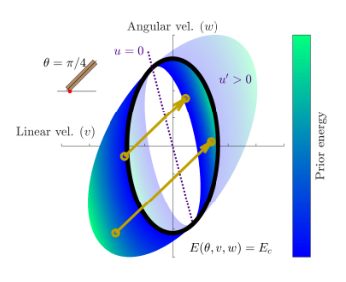
\includegraphics[width=1\columnwidth]{images/相图}
	\caption{相图\cite{c3}}
	\label{fig:P2}%\label置于\caption后,否则可能报错
\end{figure}
其中黑色的椭圆代表不等式1,外层的椭圆代表不等式2,此外由于约束$u'<0$,相图只存在对称的一般具有物理意义.

于是我们可以分别求出两个椭圆的面积:
\begin{equation}
S_{1}=2 \pi g \sqrt{\frac{m}{I}} \cdot\left(z^{*}-z_{\min }(\theta)\right) .
\end{equation}
\begin{equation}
S_{2}=\frac{2 \pi g\left(z^{*}-z_{\min }(\theta)\right)\left(I+m y^{2}\right)}{\sqrt{\left(I \gamma^{2}+m y^{2}\right)\left(I y^{2} \gamma^{2}+\frac{I^{2}}{m}\right)-I^{2} y^{2}\left(1-\gamma^{2}\right)^{2}}}
\end{equation}
对不同状态的$\theta$   ,其在相空间的面积代表其概率密度(乘上一个因子$A$是对量纲进行处理),即:
\begin{equation}
\begin{aligned}
\rho(\theta) &=\frac{m I}{A^{2}} \frac{\left.(S_{2}-S_{1}\right)}{2} \\
&=\frac{\pi m^{3 / 2} g \sqrt{I}}{
	A 
	^{2}} \cdot \frac{1-\gamma}{\gamma} \cdot\left(z^{*}-z_{\min }(\theta)\right)
\end{aligned}
\end{equation}
(其中$ A$为一个带量纲的常数,乘上的因子后续会消掉)

由求出的概率密度,再根据其对称性,可以求出理论上落在边缘的概率:
\begin{equation}
\begin{aligned}
P_{E} &=\frac{\int_{\theta=0}^{\theta=\theta_{c}} \rho(\theta) d \theta}{\int_{\theta=0}^{\theta=\pi / 2} \rho(\theta) d \theta}
=\frac{\theta_{c}-\sin \left(\theta_{c}\right)}{\pi / 2-\left(\sin \left(\theta_{c}\right)+\cos \left(\theta_{c}\right)\right)}
\end{aligned}
\end{equation}
\subsection{模型选择}
在模型选择的贝叶斯公式中,我们首先计算模型的后验概率$M_{i}$      给定数据 $D$   和任何其他信息  $I$  .由多变量的贝叶斯公式:
\begin{equation}
P\left(M_{i} \mid D, I\right)=\frac{P\left(M_{i} \mid I\right) P\left(D \mid M_{i}, I\right)}{P(D \mid I)}
\end{equation}
查看它们的比率,以检查每个模型的相对概率(即一个模型与另一个模型的概率)
\begin{equation}
\begin{gathered}
\frac{P\left(M_{i} \mid D, I\right)}{P\left(M_{j} \mid D, I\right)}=\frac{P\left(M_{i} \mid I\right) P\left(D \mid M_{i}, I\right)}{P\left(M_{j} \mid I\right) P\left(D \mid M_{j}, I\right)} \\
=\frac{P\left(M_{i} \mid I\right) L\left(M_{i}\right)}{P\left(M_{j} \mid I\right) L\left(M_{j}\right)}
\end{gathered}
\end{equation}
其中   $L$  为相应的似然函数,我们此处使用最大似然估计的方法来确定各模型的可信程度.

如果我们给每个模型分配相等的先验概率$\frac{P(M_i|I)}{P(M_j|I)}=1$,
那么后验概率的比率就变成了概率的比率  $\frac{L(M_i)}{L(M_j)}$.

利用二项分布的似然函数公式:
\begin{equation}
\begin{gathered}
\log L\left( M_i \right) =\sum{\log}n!-\log r!-\log\mathrm{(}n-r)
\\
+r\log p+(n-r)\log\mathrm{(}1-p)
\end{gathered}
\end{equation}
$n$是翻转次数,$r$    是边缘着陆次数,  $p$  是该模型预测的侧面朝上的概率.
\section{模拟}
模拟目的:
\begin{enumerate}
	\item 补充实验无法用高径比连续的一系列骰子进行实验的漏洞.
	\item 印证理论,检验理论的正确性.
	\item 与实验相互对照,检测实验误差.
\end{enumerate}
使用THREE.js构建三维环境,Cannon.js作为物理引擎,设置重力加速度,体积,质量,R/H,落下高度和初始角速度作为参量.
\begin{figure}[h]%
	\centering
	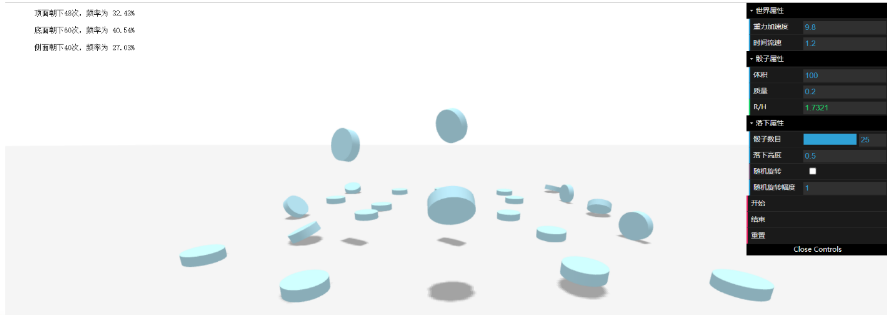
\includegraphics[width=0.8\columnwidth,height=0.15\textheight]{images/模拟场景}
	\caption{模拟场景图}
	\label{fig:P2}%\label置于\caption后,否则可能报错
\end{figure}
通过模拟与理论结合,绘制出对比图:
\begin{figure}[h]%
	\centering
	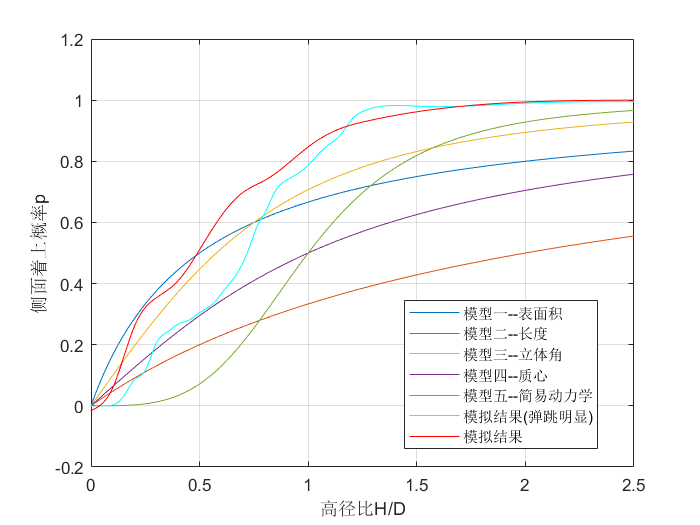
\includegraphics[width=1.1\columnwidth]{images/实验理论对比}
	\caption{模拟与理论对比}
	\label{fig:P2}%\label置于\caption后,否则可能报错
\end{figure}
\section{实验}
\label{sec:Experiment}
实验目的:
\begin{enumerate}
	\item 检验理论模型和模拟的正确性.
	\item 通过有限次实验测算出的数据与理论模型进行拟合进而修正模型.
	\item 寻找可能满足理论目标的参数组合.
\end{enumerate}
实验器材:不同高径比的亚克力,金属质地以及木质骰子(共五种材料),高径比标记在上侧(从上到下依次为亚克力,铁,铝,木头以及铜(见附录)).


给出骰子的测量不确定度:
%\begin{table}[h]                              
	%\begin{tabular}{|c|r|l}\hline
		%高径比&A类不确定度	\\ \hline
		%0.420&0.002\\\hline
		%0.621&0.001\\\hline
		%0.753&0.001\\\hline
	       % 0.823 &0.002\\\hline
	      % 1.029 &0.001\\\hline
	     %   1.231&0.001\\\hline
	      % 1.356 &0.001\\\hline
	     %  1.412&0.001\\\hline      
	%\end{tabular}
%\caption{亚克力不确定度}
%\end{table}
%\begin{table}[h]
	%\begin{tabular}{|c|r|l}\hline
		%高径比&A类不确定度	\\ \hline
		%0.401&0.003\\\hline
		%0.567&0.001\\\hline
		%0.606&0.001\\\hline
		%0.736 &0.001\\\hline
		%0.801 &0.004\\\hline                                    %修改人 任权东,修改时间2022.9.4晚23:49
		%1.002&0.002\\\hline
		%1.201 &0.001\\\hline
		%1.335&0.002\\\hline 
		%1.405&0.004\\\hline     
	%\end{tabular}
	%\caption{金属骰子不确定度}
%\end{table}

\begin{table}[h]
	\centering
\begin{tabular}{cc}
  \toprule[1.5pt]
  高径比  & A类不确定度 \\
  \midrule[0.75pt]
  0.420 & 0.002 \\
  0.621 & 0.001 \\
  0.753 & 0.001 \\
  0.823 & 0.002 \\
  1.029 & 0.001 \\
  1.231 & 0.001 \\
  1.356 & 0.001 \\
  1.412 & 0.001 \\
  \bottomrule[1.5pt]
\end{tabular}
\caption{亚克力不确定度}
\end{table}

\begin{table}[h]
	\centering
\begin{tabular}{cc}
  \toprule[1.5pt]
  高径比  & A类不确定度 \\
  \midrule[0.75pt]
  0.401 & 0.003 \\
  0.567 & 0.001 \\
  0.606 & 0.001 \\
  0.736 & 0.001 \\
  0.801 & 0.004 \\
  1.002 & 0.002 \\
  1.201 & 0.001 \\
  1.335 & 0.002 \\
  1.405 & 0.004 \\
  \bottomrule[1.5pt]
\end{tabular}
\caption{金属骰子不确定度}
\end{table}


\textbf{实验结果}

\begin{figure}[h]%
	\centering
	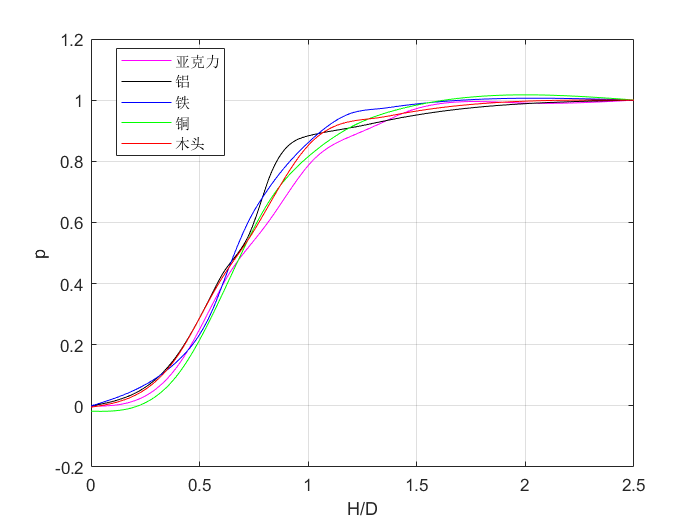
\includegraphics[width=1\columnwidth]{images/不同材质}
	\caption{不同材质骰子实验结果}
	\label{fig:P2}%\label置于\caption后,否则可能报错
\end{figure}
\begin{figure}[h]%
	\centering
	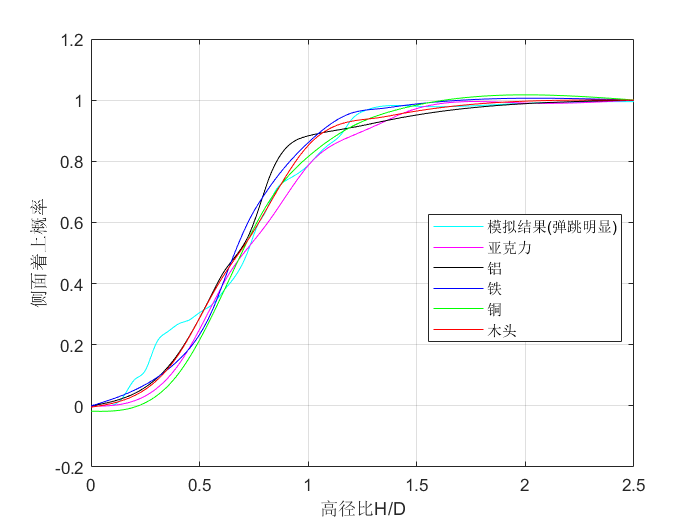
\includegraphics[width=1\columnwidth]{images/模拟(弹跳)}
	\caption{模拟与实验的对比图(弹跳明显)}
	\label{fig:P2}%\label置于\caption后,否则可能报错
\end{figure}

从实验结果图来分析:\textbf{各材料不同高径比得到的侧面朝上概率相近,且弹跳模型模拟与实验较为贴近.}

\subsection{与五个模型的对比}


仅从图片的形状与趋势分析,\textbf{模型三与模型五与实验结果有着较高的适配度},但两者与实验结果间仍存在误差.故使用似然函数对其合理性进行评估(对比图见附录).
%\begin{table}[h]
	%\begin{tabular}{|c|r|l}\hline
		%模型&似然函数值	\\ \hline
		%表面积模型&-1027\\\hline
		%长度模型&-3795\\\hline
		%立体角模型&-1225\\\hline
		%质心模型 &-2474\\\hline
		%简易运动学模型 &-93\\\hline    
	%\end{tabular}
	%\caption{各模型似然函数值}             %修改人:任权东  修改时间:2022.9.4 23:56
%\end{table}

\begin{table}[h]
	\centering
\begin{tabular}{cc}
  \toprule[1.5pt]
  模型  & 似然函数值 \\
  \midrule[0.75pt]
  表面积模型     &      -1027 \\
  长度模型       &      -3795 \\
  立体角模型     &      -1225 \\
  质心模型       &      -2474 \\
  简易运动学模型 &        -93 \\

  \bottomrule[1.5pt]
\end{tabular}
\caption{各模型似然函数值}
\end{table}


结论:\textbf{仅从趋势来看,模型5为最佳模型.}

用似然函数仅能排除掉模型二与模型四,无法完全排除模型一,三,五.其也有在物理上的合理性.我们假设三个组合能通过线性叠加得到最后的结果,具体表述如下:
\begin{equation}
y=ax_1+bx_2+cx_3
\end{equation}
  $y$ 代表现实中的骰子侧面着上的概率,  $  x_1,x_2,x_3 $                  分别代表模型一,三,五的概率.
  
 \begin{figure}[h]%
 	\centering
 	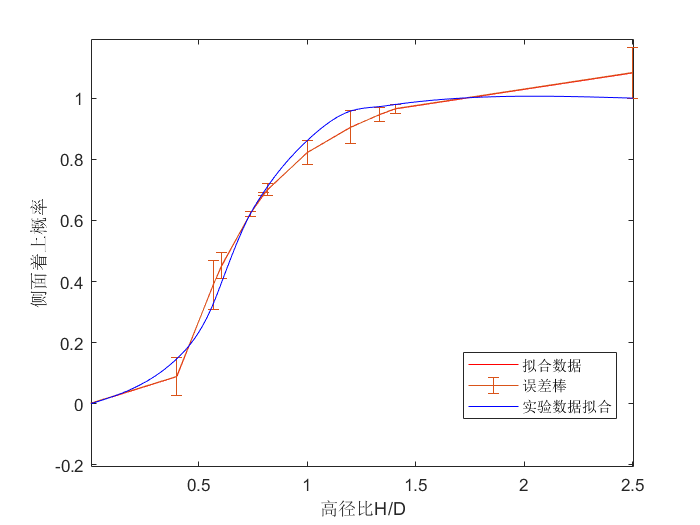
\includegraphics[width=0.8\columnwidth]{images/线性拟合误差棒}
 	\caption{线性拟合结果}
 	\label{fig:P2}%\label置于\caption后,否则可能报错
 \end{figure}

\begin{table}[h]
	\centering
\begin{tabular}{ccc}
  \toprule[1.5pt]
  \diagbox{概率}{模型}   & 弹跳    &  不弹跳 \\
  \midrule[0.75pt]
   $P_E=\frac{1}{3}$    & 0.535   &  0.641   \\
   $P_E=\frac{1}{2}$    & 0.354   &  0.577  \\
  \bottomrule[1.5pt]
\end{tabular}
\caption{结果预测}
\end{table}



拟合结果为:
\begin{equation}
y=-5.3879x_1+6.7528x_2-0.7216x_3
\end{equation}

拟合优度为:$R^2=0.9817$.

由于数据量的原因,该结果在前端和后端拟合结果较差,但在概率0.2-0.9的部分与实验结果符合的较好,由此我们可以对最终结果进行预言.
%\begin{table}
%\begin{tabular}{|l|c|c|c|}
%	\hline
%	\diagbox{概率}{模型} & 弹跳 & 不弹跳  \\
%	\hline
%$P_E=\frac{1}{3}$ & 0.535 & 0.641  \\
%	\hline
%	$	P_E=\frac{1}{2}	$ & 0.354 & 0.577  \\   % 注意方向参数是[]
%	\hline
%\end{tabular}
%\caption{结果预测}                                             修改人:任权东  修改时间:2022.9.5 0:17
%\end{table}


(表内二三列指的是$
\frac{H}{D}$)

\textbf{误差分析}

可能的误差来源: 
      
1.系统误差:        

在模型上我们简化为坠落平面为无摩擦平面上,但实际器材无法达到预期.   

    
2.人员和器材误差:   

圆柱形骰子的高,直径使用精度为0.02mm的游标卡尺测量,存在一定误差.       
骰子在进行多次的实验时出现了一定情况的磨损.       

实验人员在实验中不可避免出现一些误差.

\textbf{不足与展望}

1:探究的模型做了诸多简化,无法确定其中忽略的因素是否会对结果产生重大影响.

2:实验次数不够,与大数定律有一定偏差.

3:理论结果与实验结果仍存在着一定的误差.
%致谢,参考文献与背景信息部分=========================================================
\section*{致谢}
探究小组成员:谭帆驰\quad  丁俊翔\quad  杨超毅\quad  杜溪翔 \quad 邱卓伦  

此外,尤其鸣谢物理实验创新基地(IBPE)的各成员的协作,比赛主办方和指导老师,以及参赛同学.
%致谢部分记得改过来好吗!!!!仔细看看模板的内容!!!!!!!!!!!!!!!!!!


%背景信息
\Note{BlueNoteBackground}{
  {\textbf{Your Name}} 谭帆驰\\
  {\textbf{Address:}} School of Physics, Huazhong University of Science and Technology\\
  {\textbf{Email:}} U202010215@hust.edu.cn
}
%写上你们的背景信息呀!!!!!!这上面的背景信息都是乱填的呀!!!!!!!!!!!
%觉得多余的可以删去,觉得不够的也可以增添别的背景信息!!!!!!!!!!!!!!!!!!!!!!!!!!!!

\section*{参考文献}
\begin{thebibliography}{2}

\bibitem{c1}Teaching Bayesian Model Comparison With theThree-Sided Coin[J]The American Statistician Scott R Kuindersma  Brian S Blais (2007)

\bibitem{c2}Probability of a tossed coin landing on edge[J]PHYSICAL REVIEW E Daniel B.Murray  Scott W. Teare(1993.9)

\bibitem{c3}Exact edge landing probability for the bouncing coin toss and the three-sided die problem[J]Llu´ıs Hern´andez-Navarro and Jordi Pi˜nero(2021.4)
\end{thebibliography}
\section{附录}
\subsection{实验器材}
\begin{figure}[H]%
	\centering
	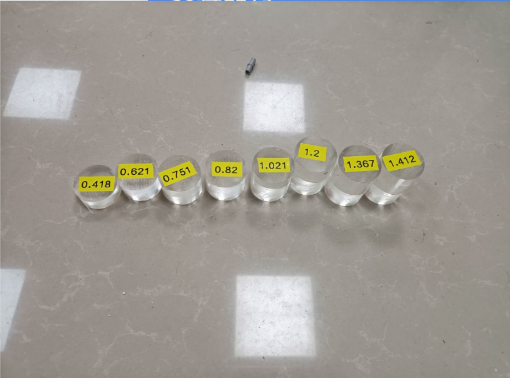
\includegraphics[width=1.1\columnwidth]{images/亚克力}
	\caption{亚克力}
	\label{fig:P2}%\label置于\caption后,否则可能报错
\end{figure}
\begin{figure}[H]%
	\centering
	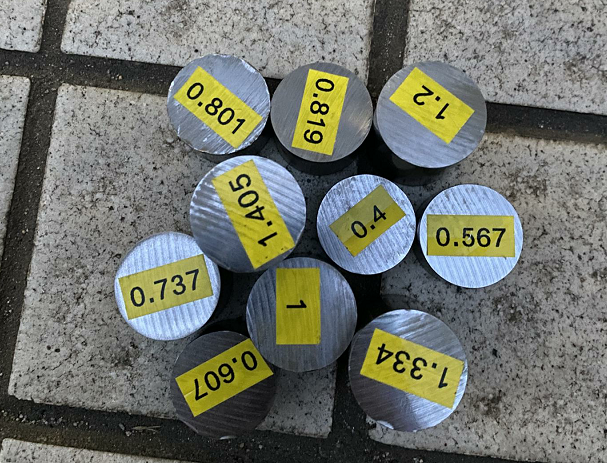
\includegraphics[width=1.1\columnwidth]{images/铁}
	\caption{铁}
	\label{fig:P2}%\label置于\caption后,否则可能报错
\end{figure}
\begin{figure}[H]%
	\centering
	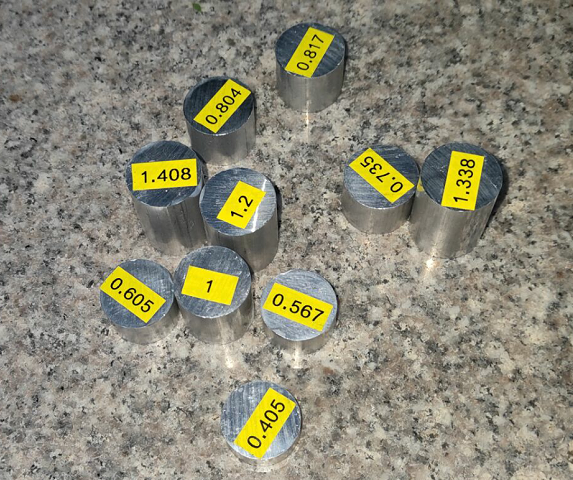
\includegraphics[width=1\columnwidth]{images/铝}
	\caption{铝}
	\label{fig:P2}%\label置于\caption后,否则可能报错
\end{figure}
\begin{figure}[H]%
	\centering
	\includegraphics[width=1\columnwidth]{images/木}
	\caption{木}
	\label{fig:P2}%\label置于\caption后,否则可能报错
\end{figure}
\begin{figure}[H]%
	\centering
	\includegraphics[width=1\columnwidth]{images/铜}
	\caption{铜}
	\label{fig:P2}%\label置于\caption后,否则可能报错
\end{figure}
%\end{CJK}
\subsection{模型对比}
\begin{figure}[H]%
	\centering
	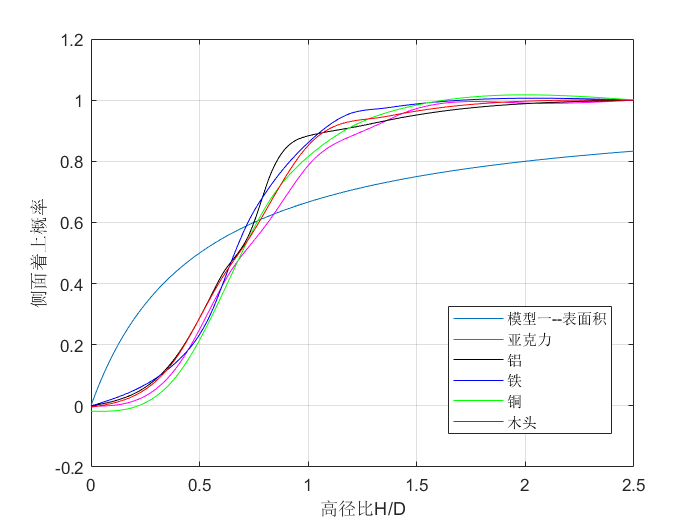
\includegraphics[width=1\columnwidth]{images/比较1}
	\caption{与模型一的对比图}
	\label{fig:P2}%\label置于\caption后,否则可能报错
\end{figure}
\begin{figure}[H]%
	\centering
	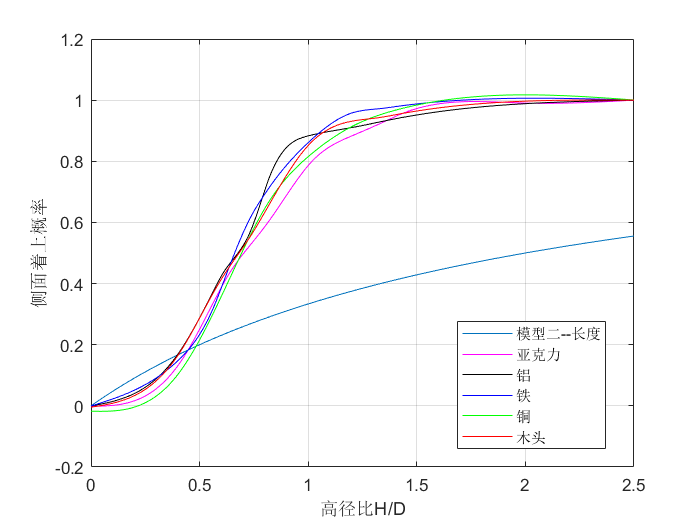
\includegraphics[width=1\columnwidth]{images/比较2}
	\caption{与模型二的对比图}
	\label{fig:P2}%\label置于\caption后,否则可能报错
\end{figure}
\begin{figure}[H]%
	\centering
	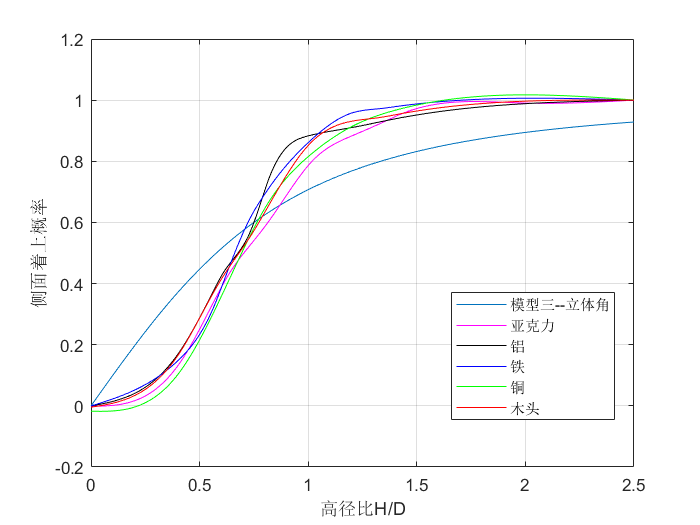
\includegraphics[width=1\columnwidth]{images/比较3}
	\caption{与模型三的对比图}
	\label{fig:P2}%\label置于\caption后,否则可能报错
\end{figure}
\begin{figure}[H]%
	\centering
	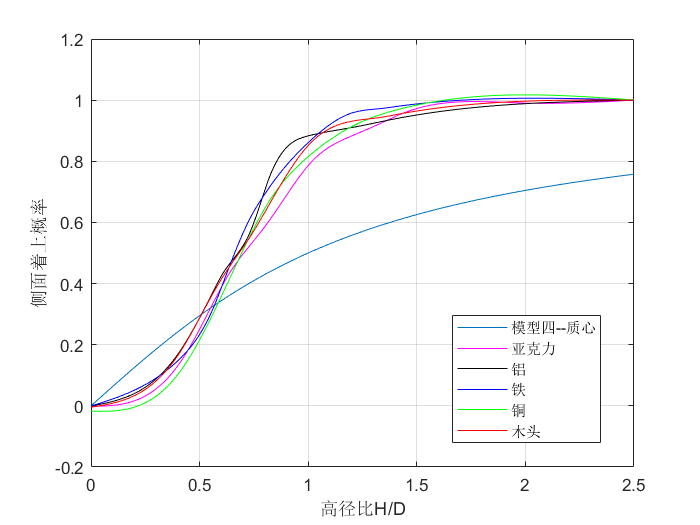
\includegraphics[width=1\columnwidth]{images/比较4}
	\caption{与模型四的对比图}
	\label{fig:P2}%\label置于\caption后,否则可能报错
\end{figure}
\begin{figure}[H]%
	\centering
	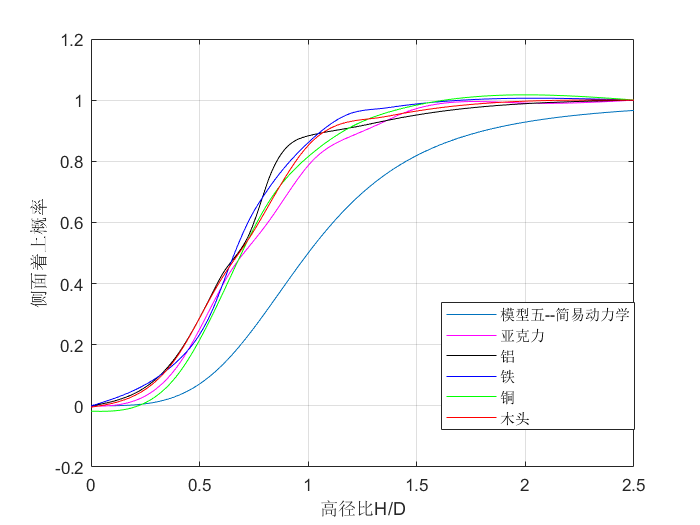
\includegraphics[width=1\columnwidth]{images/比较5}
	\caption{与模型五的对比图}
	\label{fig:P2}%\label置于\caption后,否则可能报错
\end{figure}
\end{document}